\documentclass[graphics]{beamer}
\usepackage{xcolor}
\usepackage{graphicx}
\usepackage{verbatim}
\usepackage{wrapfig}
\usepackage{tabularx}
\usepackage{multirow}
\usepackage{amssymb}
\usepackage{pifont}
\usepackage{tikz}
\def\Checkmark{\tikz\fill[scale=0.2](0,.35) -- (.25,0) -- (1,.7) -- (.25,.15) -- cycle;} 

\useoutertheme{shadow}
%\usecolortheme{orchid}
\usecolortheme{seahorse}
\newcommand{\cmark}{\text{\ding{51}}}
%\newcommand*{\GtrSim}{\smallrel\gtrsim}

% math commands
\newcommand{\be}{\begin{eqnarray}}
\newcommand{\ee}{\end{eqnarray}}
\newcommand{\beq}{\begin{equation}}
\newcommand{\eeq}{\end{equation}}
\def\simless{\mathbin{\lower 3pt\hbox
      {$\rlap{\raise 5pt\hbox{$\char'074$}}\mathchar"7218$}}}
\def\simgreat{\mathbin{\lower 3pt\hbox
      {$\rlap{\raise 5pt\hbox{$\char'076$}}\mathchar"7218$}}} %> or of order

% variables

\def\toonscale{0.45}
\def\mboxy#1{\mbox{\small #1}}

\defbeamertemplate*{title page}{customized}[1][]
{
  \usebeamerfont{title}\inserttitle\par
  \usebeamerfont{subtitle}\usebeamercolor[fg]{subtitle}\insertsubtitle\par
  \bigskip
  \usebeamerfont{author}\insertauthor\par
  \usebeamerfont{institute}\insertinstitute\par
  \usebeamerfont{date}\insertdate\par
  \usebeamercolor[fg]{titlegraphic}\inserttitlegraphic
}
\begin{comment}
\AtBeginSection[]{
  \frame{
    \frametitle{Outline}
    \tableofcontents[currentsection]
  }
}
\end{comment}


\title{\textcolor{white}{Cosmology with FRBs}}
%\subtitle{}
\author[U. Pen]{{
\textcolor{green}{\small Ue-Li Pen, CITA}
}
\\[8mm] 
}
\date{\textcolor{green}{September 4, 2019}}


\begin{document}

\frame{
\vspace{-0.5in}
\begin{center}  
%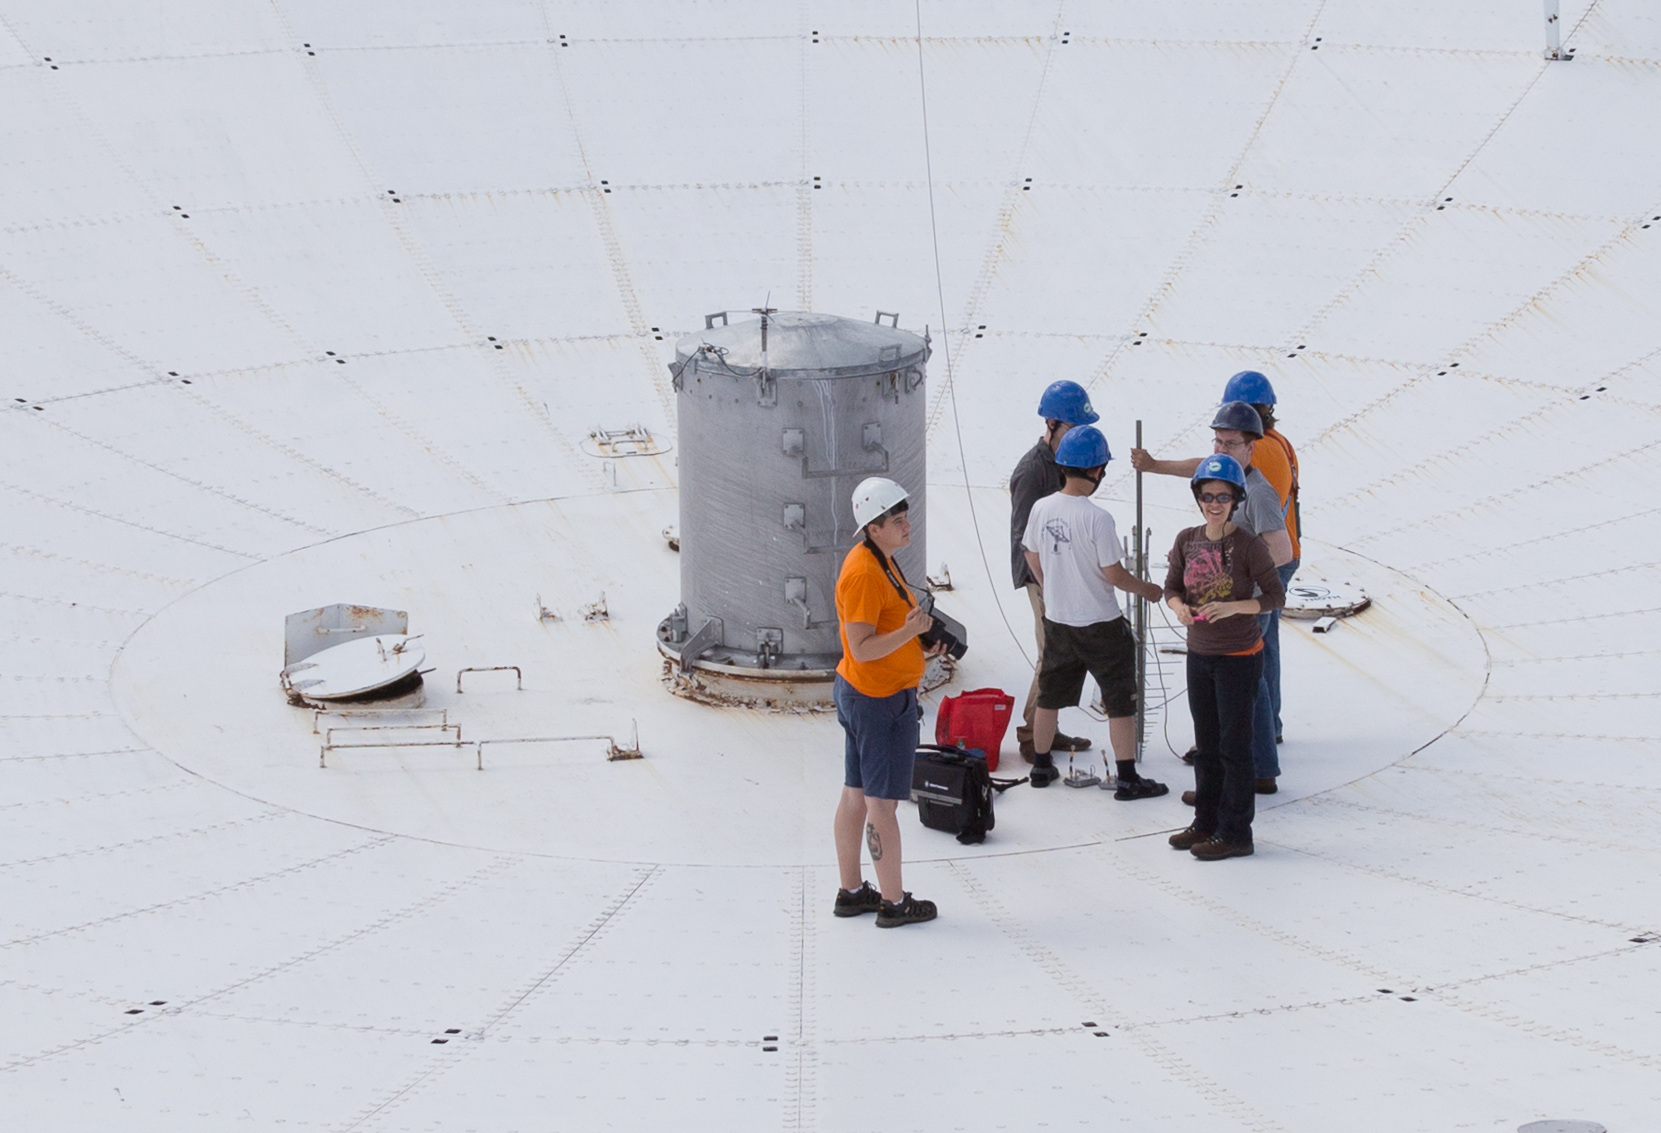
\includegraphics[width=4.4in]{Figures/IMG-0438-by-Andre-cropped.jpg}
\end{center}
\begin{picture}(320,250)
\put(-35,6){
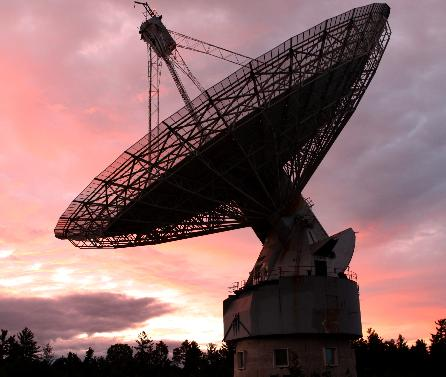
\includegraphics[width=5.1in]{Figures/IMG-7749-ARO-crop.JPG}
}
\end{picture}
\vspace{-4in}
\\
%image credit: NRAO/AUI/NSF
\\
\vspace{1in}
\titlepage
}

%\section*{Introduction}
\section{Introduction}

\begin{comment}
  \subsection{Outline}

  \frame{
    \frametitle{Outline}
    \tableofcontents
  }
\end{comment}

  \frame{
    \frametitle{Overview}
    \begin{itemize}
      \item FRBs: what we currently know
      \item misconceptions
      \item precision
    \end{itemize}
  }

  \frame{
    \frametitle{FRB state}
    \begin{itemize}
      \item occur all-sky, with thousands of bright bursts per day,
        and many more faint ones: roughly Euclidean fluence, $N(>S)
        \propto S^{-1.5}$.
      \item many ($>11$), perhaps all, repeat (1908.03507).
      \item some localized, distance $\sim $Gpc
    \end{itemize}
  }

  \frame{
    \frametitle{Instrumentation revolution}
    \begin{itemize}
    \item CHIME: FFT Telescope (Tegmark and Zaldarriaga 2009++)
    \item disruptive technology: orders of magnitude more events than
      all existing and planned radio telescopes, at small fraction of cost
    \item no moving parts, software telescope:  utilize N log N beam
      forming (FFT), N log N  DM search, builds on information
      revolution technology: efficient low cost receivers (cell
      phones), computing.
    \item opens path to much more ambitious surveys.
    \end{itemize}
  }


  \frame{
    \frametitle{Cosmological implications: misconceptions}
    \begin{itemize}
    \item many papers using 'standard' DM: dark energy/EoS, baryon
      evolution
    \item covariant (degenerate) with likely evolution of host environment
    \end{itemize}
  }

  \frame{
    \frametitle{Cosmological implications: likely initial results}
    \begin{itemize}
    \item cross correlation baryon inventory (McQuinn 2014++)
    \item likely to probe intergalactic medium equation of state
    \item requires precision positions and/or redshifts
    \end{itemize}
  }
  \frame{
    \frametitle{Underappreciated: Coherence}
    \begin{itemize}
    \item most FRB's in coherent/eikonal limit
    \item multi-path propagation due to gravitational and plasma
      lensing
    \item dominant (sole?) population of extragalactic coherent sources
      exhibiting interference (scintillation!)
    \item path length measured to $ \delta L\sim$ nanoseconds
    \item dimensionless strain $h=\delta L/L\sim 10^{-25}$: unique
      window on cosmic space-time metric (e.g. Yang+ 2017)
    \item special geometry, fudge factor up to $10^5$
    \end{itemize}
  }

  \frame{
    \frametitle{Multi-path lensing}
    \begin{itemize}
    \item gravitational lensing:
    \item compact objects: stars, planets (unique window on
      extragalactic planets!), black holes, dark matter.  Time delay: milli-nano seconds
    \item dark matter, substructure, self-interaction: years-milli-seconds
    \item coherent interference measures time delay to nano-seconds
    \item guaranteed to change from day to day
    \end{itemize}
  }


  \frame{
    \frametitle{Multi-plane lensing}
    \begin{itemize}
    \item compact objects: stars, planets (unique window on
      extragalactic planets!), black holes, dark matter.  Time delay: milli-nano seconds
    \item dark matter, substructure, self-interaction: years-milli-seconds
    \item coherent interference measures time delay to nano-seconds
    \item guaranteed to change from day to day
    \end{itemize}
  }

  \frame{
    \frametitle{path integrals}
    \begin{itemize}
    \item Huygens' principle: sum over all paths (same as quantum field
      theory: Fermat, Feynmann, Fresnel-Kirchhoff)
    \item highly oscillatory integrals $\int \exp[i \phi({\bf x})]d^nx$
    \item considered barely tractible in 2-d
    \item Picard-Lefshitz theory
    \end{itemize}
  }



\frame{
    \frametitle{Lens notation}
     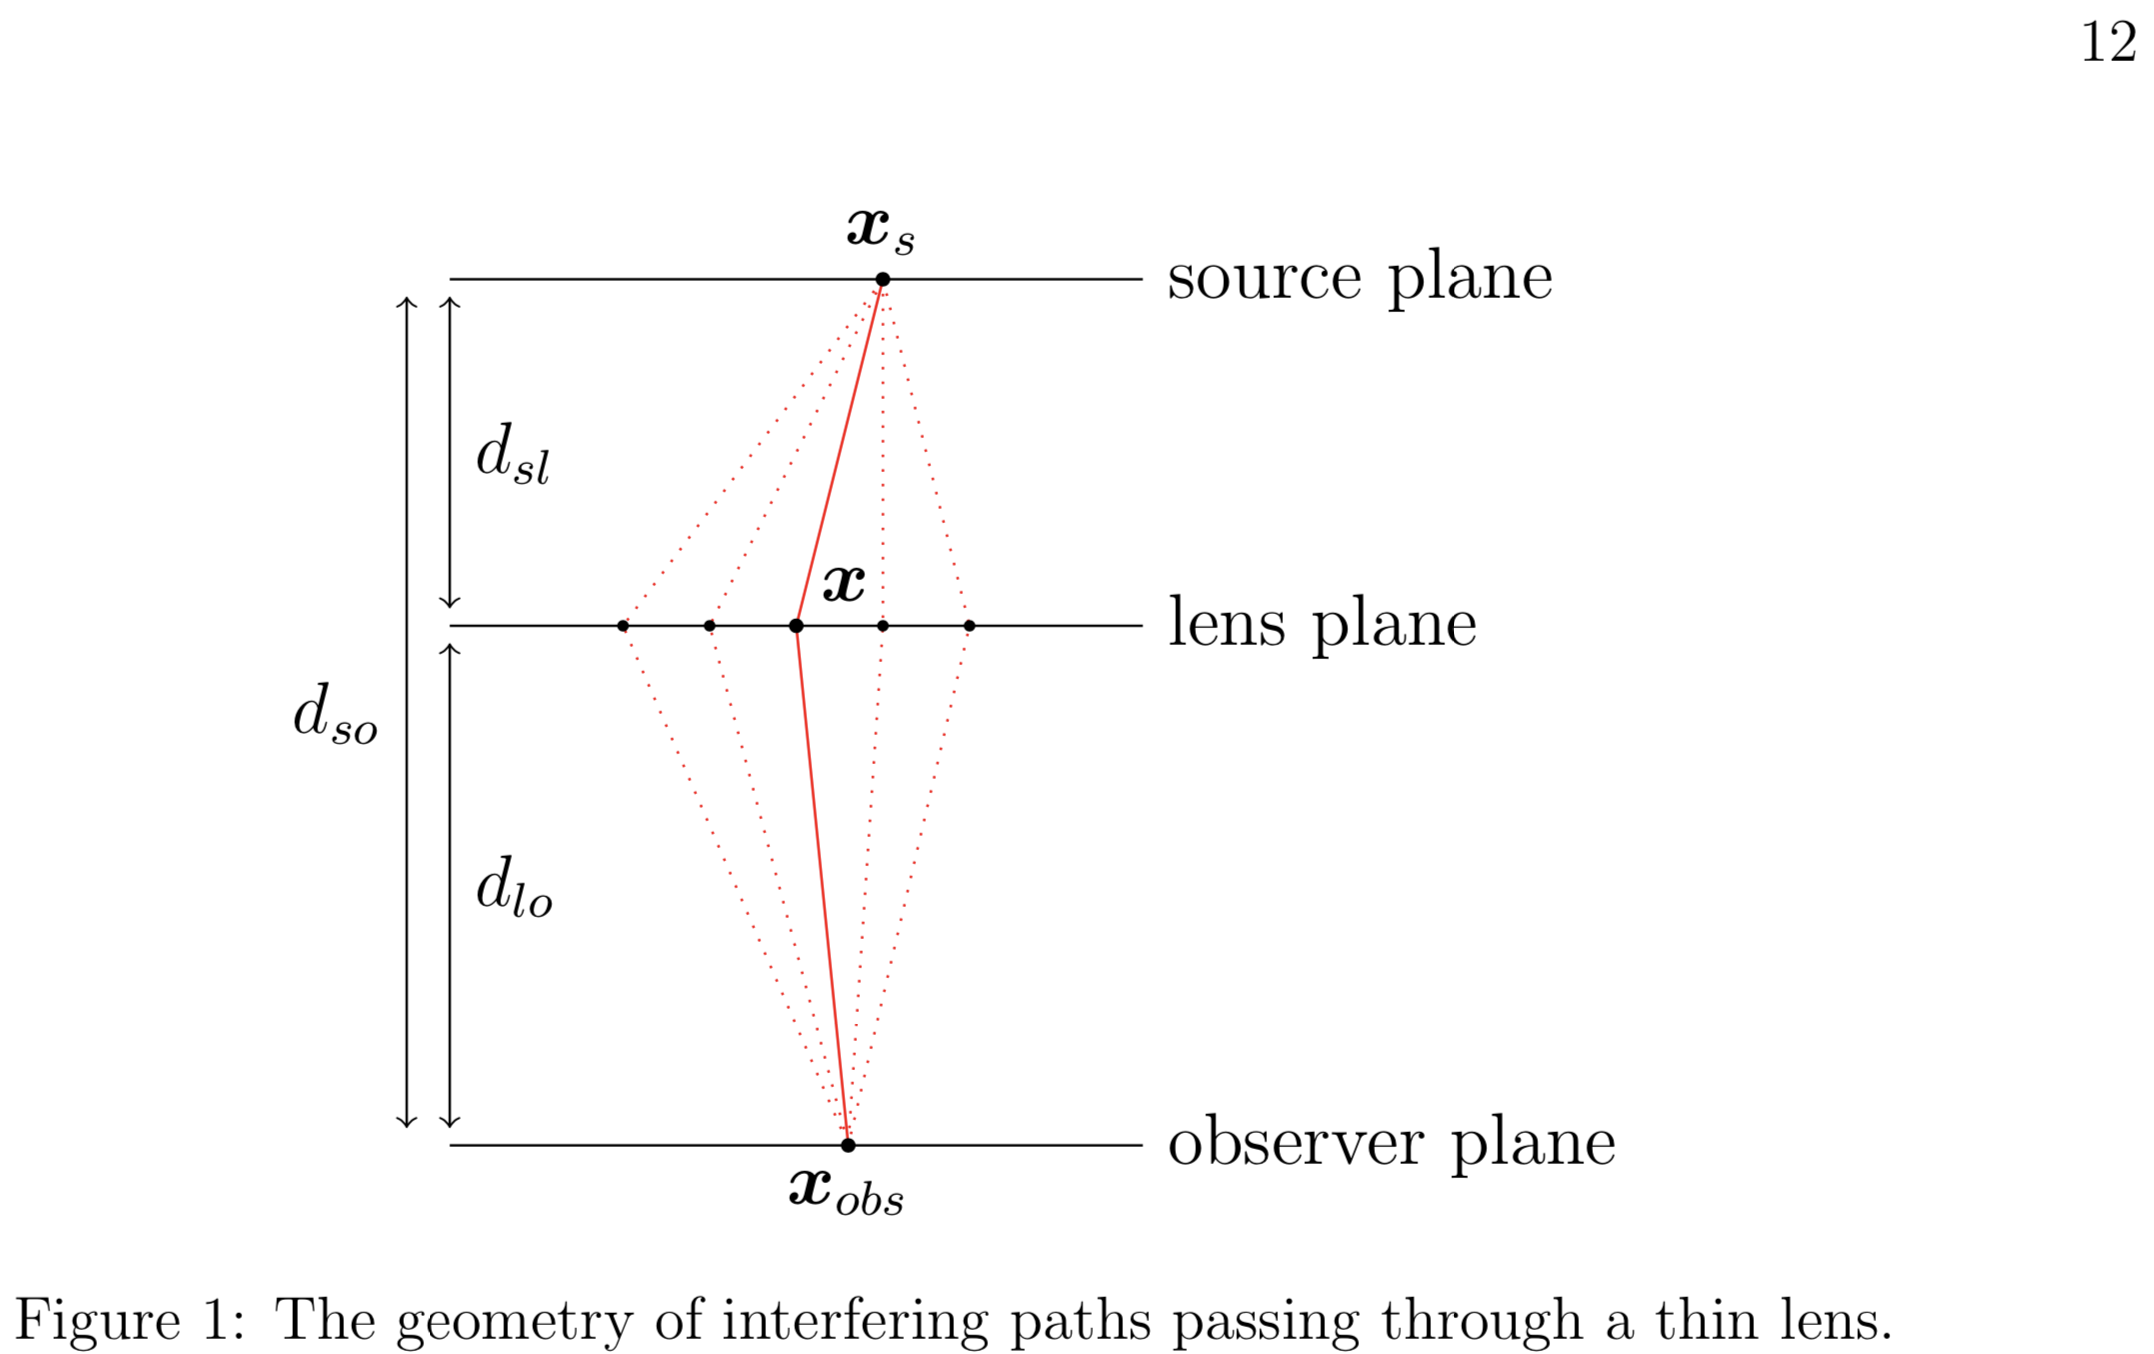
\includegraphics[width=1.01\textwidth]{Figures/lens-schematic.png}
{\hspace{-0.1in}\tiny Feldbrugge+ 2019}
}

\frame{
    \frametitle{Geometric Lens}
\begin{center}
     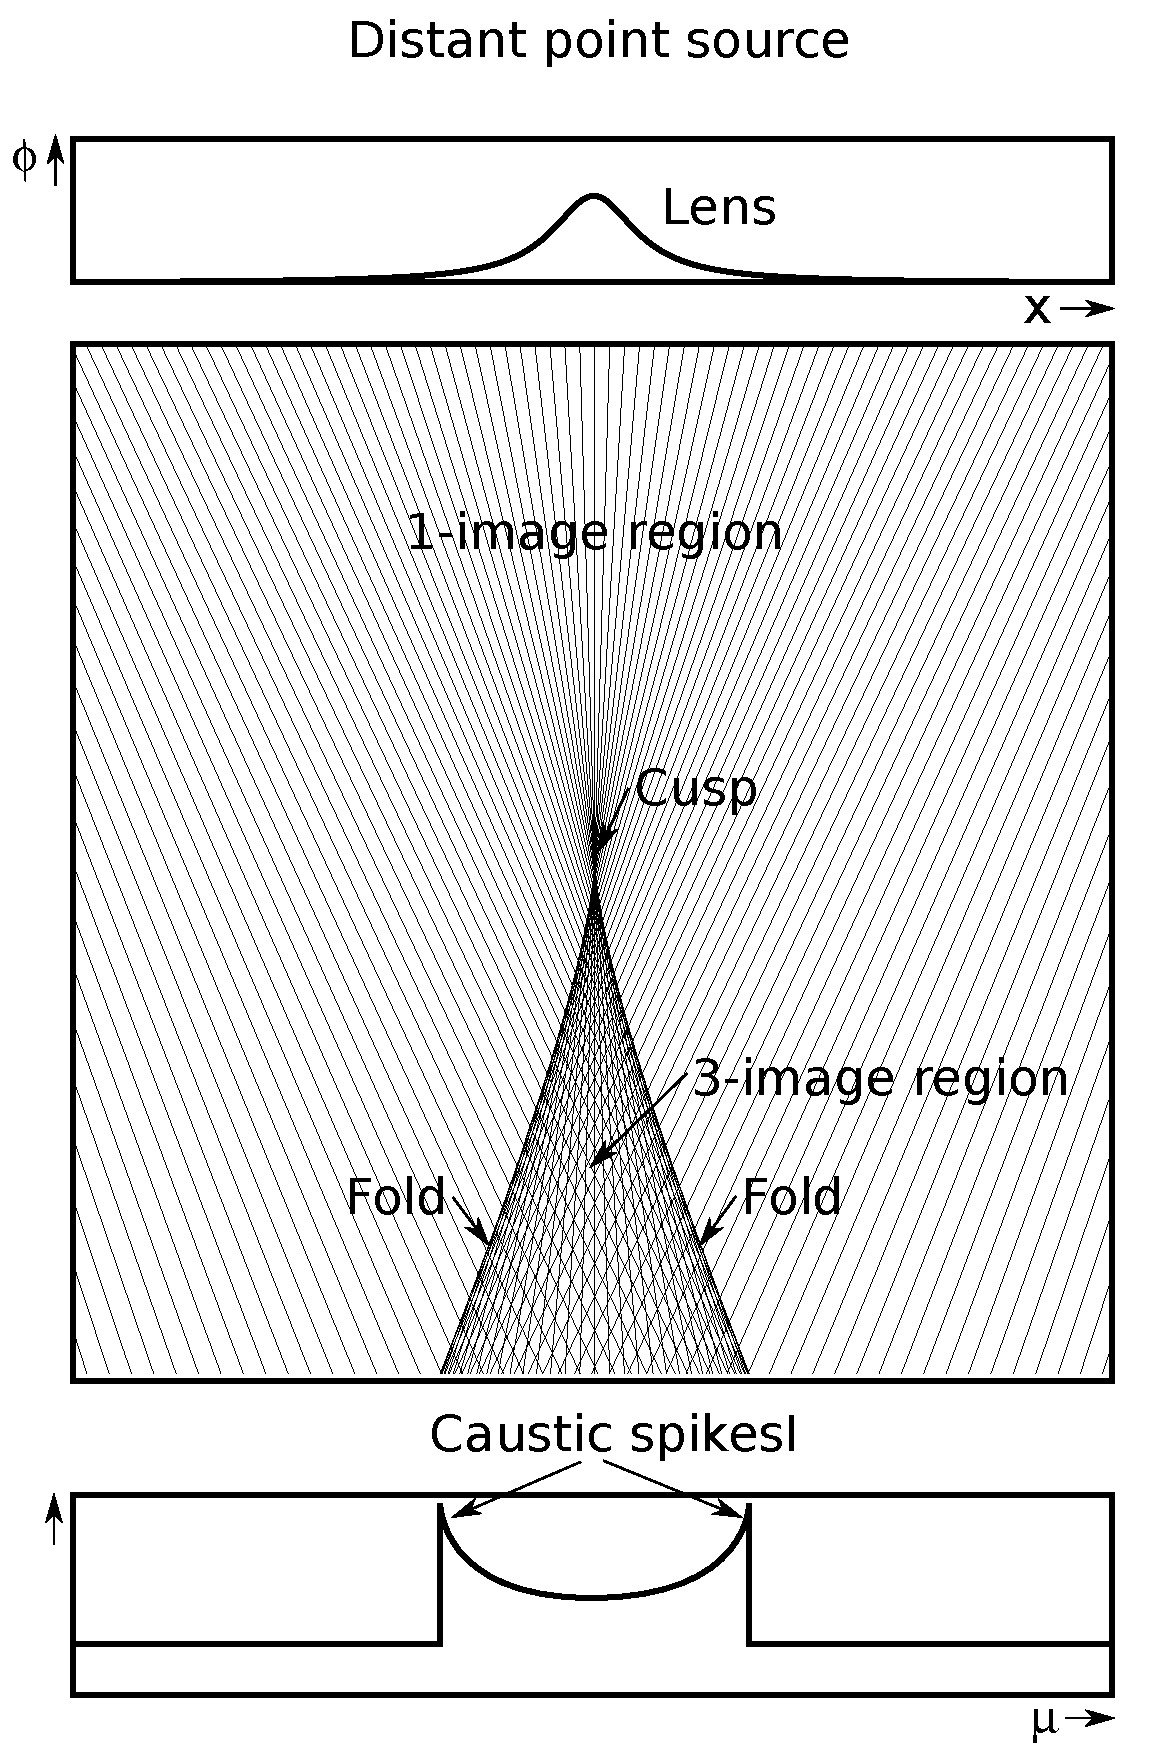
\includegraphics[width=0.45\textwidth]{Figures/GeometricOptics.pdf}
\end{center}
}
\frame{
    \frametitle{Wave Lens}
     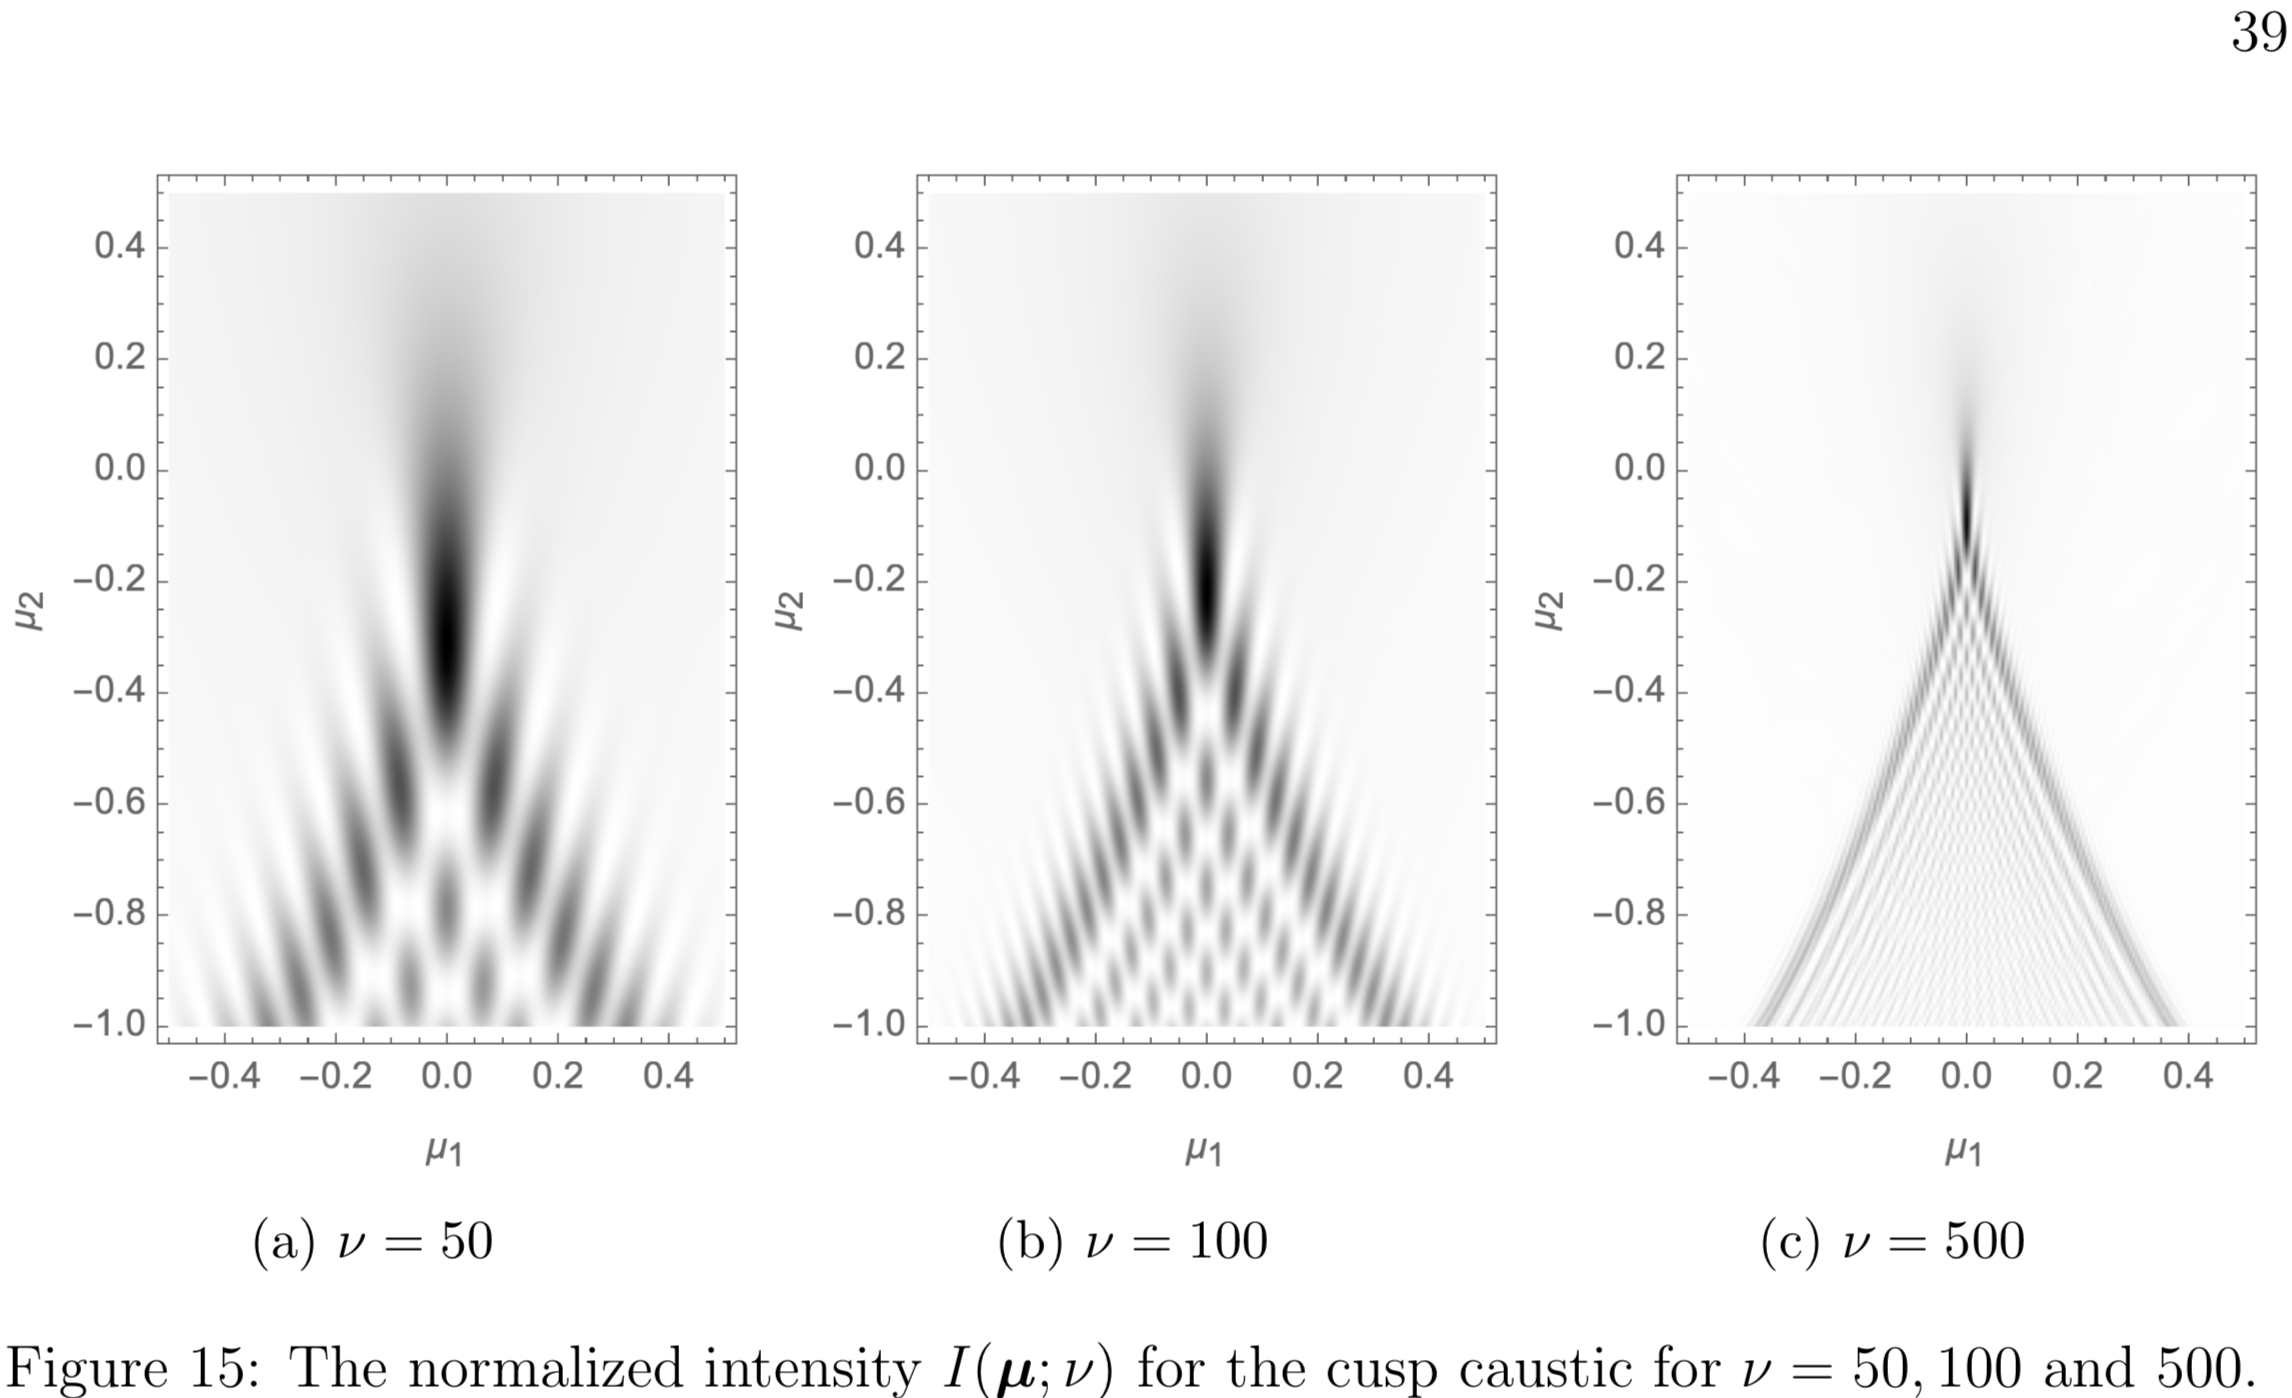
\includegraphics[width=1.01\textwidth]{Figures/wave-cusp.png}
}

\frame{
    \frametitle{Data}
     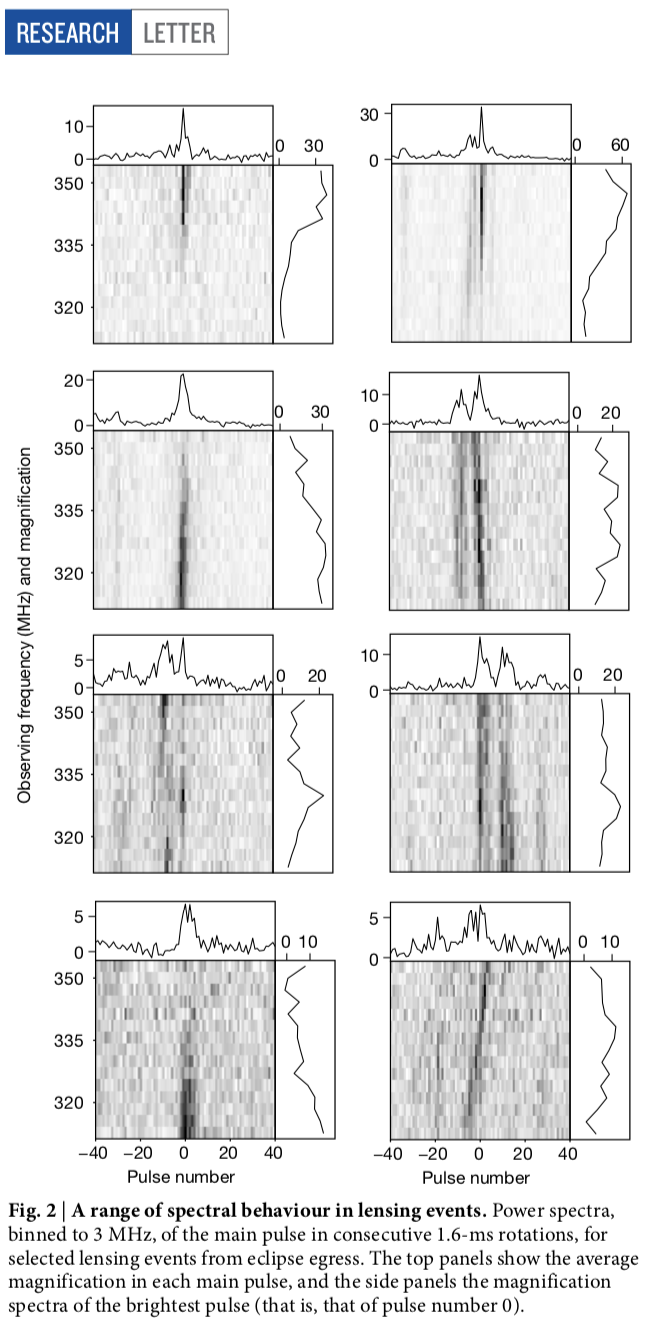
\includegraphics[width=0.38\textwidth]{Figures/b1957-lens.png}
\vspace{-0.4in}
     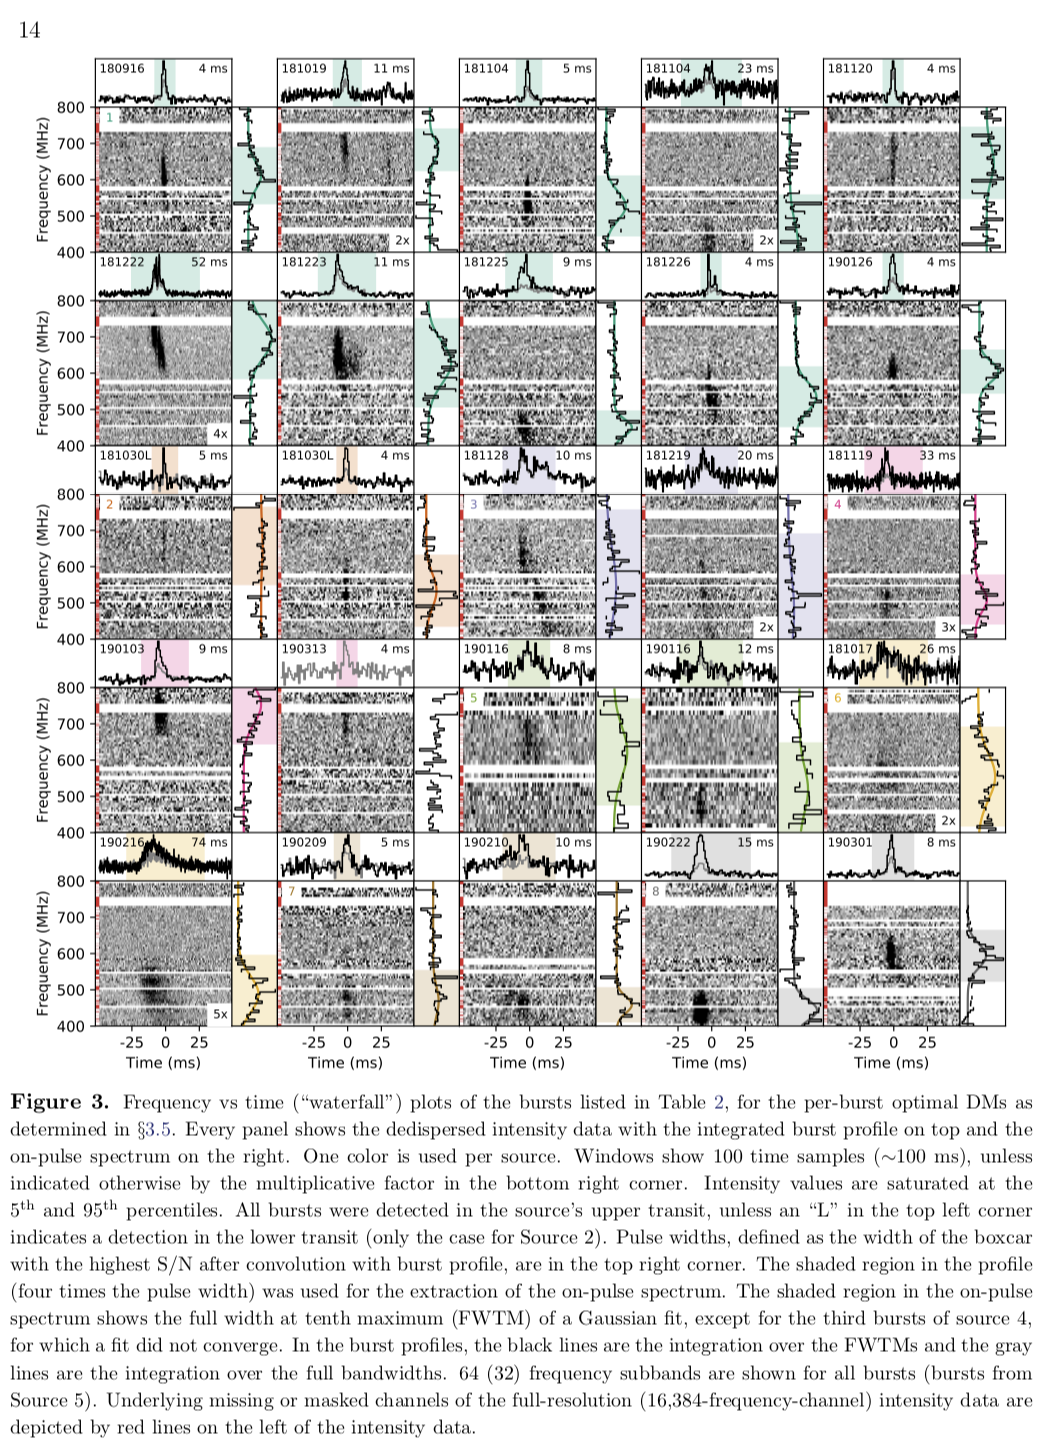
\includegraphics[width=0.52\textwidth]{Figures/frb-repeat.png}
{\tiny \hspace{-0.4in} Main et al 2018, CHIME 2019}
}


\section{FRBs}


\frame{
    \frametitle{FRB110523}
     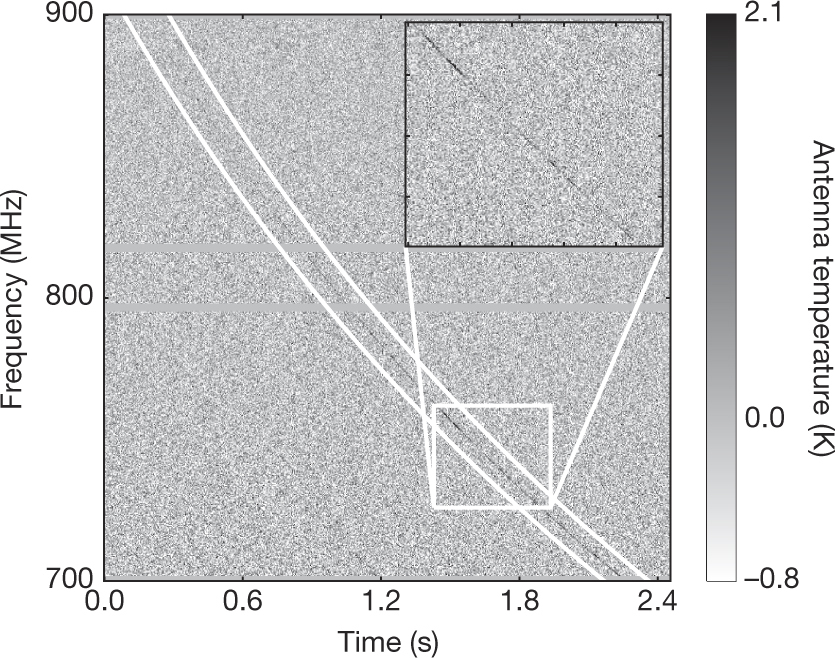
\includegraphics[width=0.8\textwidth]{Figures/nature15769-f1.jpg}

Masui et al 2015
}
\frame{
    \frametitle{Scattering}
     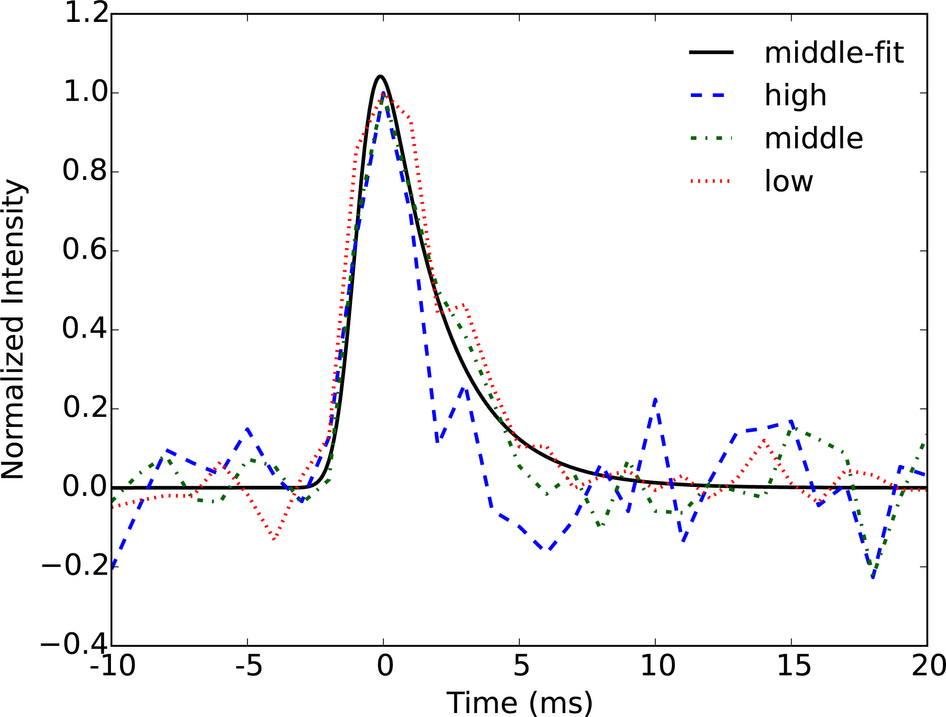
\includegraphics[width=0.8\textwidth]{Figures/nature15769-sf2.jpg}
}


\frame{
    \frametitle{Crab}
     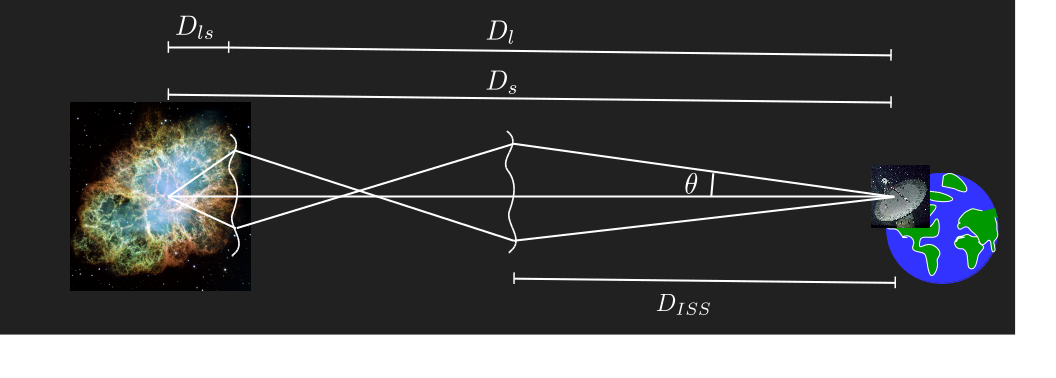
\includegraphics[width=1.1\textwidth]{Figures/TwoScreenGeometry.png}

(figure credit: R. Main)

$\tau_{\rm nebula}\gg \tau_{\rm ISM}$
}

  \frame{
    \frametitle{Two screen physics}
    \begin{itemize}
      \item FRB110523:
      \item long $\sim 1$ms: local to host
      \item short $\sim 1 \mu$s: galactic
      \item FRB121102:
      \item long $\sim 10$ns: local to host
      \item short $\sim 20 \mu$s: galactic
    \end{itemize}
  }
  \frame{
    \frametitle{interpretation}
    \begin{itemize}
    \item ms scattering is generally due multipath propagation
    \item location has been proposed in IGM (theoretically challenging) or intervening halos
    \item FRB110523 shows $\mu$s scintillation from Galactic multipath
    \item scattering tail scintillates!
    \item {\it stars twinkle, planets don't}
    \item constrains source size less than $\sim$ microarcsecond
    \item scattering screen is physically associated with FRB, not
      intergalactic or intervening
    \end{itemize}
  }

  \frame{
    \frametitle{Future possibilities}
    \begin{itemize}
    \item event rate proportionate to field of view, collecting area
    \item millions of bright FRBs per year, likely billions per year
      accessible with achievable budgets
    \item outriggers will localize all events at milli arcsecond resolution
    \item resolve some gravitaiona/plasma lenses
    \end{itemize}
  }

\section{Summary}



  \frame{
    \frametitle{Conclusion}
    \begin{itemize}
    \item coherence of FRBs underappreciated
    \item one of the most precise measurements ($10^{-25}$)
    \item wave propagation poses new theory challenges: oscillatory
      path integrals (Feldbrugge at al 2019+)

      \item Two screen scintillation/scattering: crab, FRB110523
      \item low frequency VLBI could quantify galactic screen distance,
        constrain source screen distance
      \item beginning of new era, for theory and data
    \end{itemize}
  }

\end{document}
